\documentclass[a4paper,12pt,twoside,openany]{memoir}
\setheadfoot{28pt}{1cm}

%%% DIVERSE PAKKER %%%
\usepackage{float}

% Listings til kode

\usepackage{listings}
\lstloadlanguages{[Sharp]C}
\renewcommand\lstlistingname{Code example}

\lstset{ %
language=[Sharp]C,              % the language of the code
%basicstyle=\footnotesize,      % the size of the fonts that are used for the code
numbers=left,                   % where to put the line-numbers
%numberstyle=\footnotesize,     % the size of the fonts that are used for the line-numbers
stepnumber=1,                   % the step between two line-numbers. If it's 1, each line 
                                % will be numbered
numbersep=5pt,                  % how far the line-numbers are from the code
%backgroundcolor=\color{white}, % choose the background color. You must add \usepackage{color}
showspaces=false,               % show spaces adding particular underscores
showstringspaces=false,         % underline spaces within strings
showtabs=false,                 % show tabs within strings adding particular underscores
frame=single,                   % adds a frame around the code
tabsize=2,                      % sets default tabsize to 2 spaces
captionpos=t,                   % sets the caption-position to top
breaklines=true,                % sets automatic line breaking
breakatwhitespace=false,         % sets if automatic breaks should only happen at whitespace
%title=\lstname,                % show the filename of files included with \lstinputlisting;
                                % also try caption instead of title
%escapeinside={\%*}{*)},        % if you want to add a comment within your code
%morekeywords={*,...}           % if you want to add more keywords to the set
}

% Dansk orddeling
\usepackage[english]{babel}

%Floats og [H]
\usepackage{float}

% Nummering af eksempler og sætninger
\usepackage{amsthm}
\theoremstyle{definition}
\newtheorem{example}{Example}
\newtheorem{theorem}{Theorem}

% Giver mulighed for at bruge æ, ø og å i .tex-filer
\usepackage[utf8x]{inputenc}

% Hjælper med orddeling ved æ, ø og å. Sætter fontene til at
% være ps-fonte, i stedet for bmp
\usepackage[T1]{fontenc}

% Pakke, der gør det muligt at anvende grafikfiler, samt andvende flere captions på samme figure
\usepackage{graphicx}
\usepackage{caption}
\usepackage{subcaption}

% Pakker, der kan udelades, hvis man ikke gør megen brug af matematik
\usepackage{amsmath}
\usepackage{amssymb}

% Pakke, der kan indsætte nødvendige mellemrum efter
% makro-anvendelser.
\usepackage{xspace}

% Retter forskellige bugs i LaTeX-kernen
\usepackage{fixltx2e}

% Indsæt rettelser og lignende med \fixme{...} med "final"
% i stedet for "draft" udløses en error for hver fixme,
% når der compiles.
\usepackage[footnote,draft,english,silent,nomargin]{fixme}

% Gør det muligt at definere farver.
% Se en.wikibooks.org/wiki/LaTeX/Colors for mere info.
\usepackage{color}
\usepackage[usenames,dvipsnames]{xcolor}

%Hyperlinks i indholdsfortegnelse
\usepackage{hyperref}

%Itemization i tables og andet leg
\usepackage{tabularx}
\usepackage{booktabs} % http://ctan.org/pkg/booktabs
\newcommand{\tabitem}{~~\llap{\textbullet}~~}

\hypersetup{
	bookmarks=true,  % Vis 'bookmark'-ramme.
	colorlinks=true, % True = links har farver, False = links har rammer
	citecolor=black,  % Linkfarve for referencer.
	linkcolor=black,  % Linkfarve i indholdsfortegnelse
	urlcolor=black,   % Linkfarve for eksterne URL'er.
}

%%% LITTERATURLISTE %%%
\usepackage[square,numbers]{natbib}
\usepackage{url}

%%% MARGINER %%%
\setlrmarginsandblock{3.5cm}{2.5cm}{*}	% \setlrmarginsandblock{Indbinding}{Kant}{Ratio}
\setulmarginsandblock{2.5cm}{3.0cm}{*}	% \setulmarginsandblock{Top}{Bund}{Ratio}
\checkandfixthelayout 			% Laver forskellige beregninger og sætter de almindelige længder op til brug ikke memoir pakker


%%% OTHER STUFF %%%
\newcommand{\pdf}{PDF}

\newcommand{\Z}{\ensuremath{\mathbb{Z}}\xspace}

% Kommando, der sikrer ensartede referencer til figurer

\newcommand{\figref}[1]{Figure \ref{#1}}

\newcommand{\mgd}[2]{\ensuremath{\{ #1 \mid #2 \}}}

%\newtheorem{saetning}{S�tning}
\newtheorem{definition}{Definition}




\usepackage{cleveref}
\crefname{listing}{code example}{code examples}
\usepackage{todonotes}

% Valg a kapiteludseende
\definecolor{numbercolor}{gray}{0.7}			% Definerer en farve til brug til kapiteludseende
\newif\ifchapternonum

\makechapterstyle{jenor}{									% Definerer kapiteludseende -->
  \renewcommand\printchaptername{}
  \renewcommand\printchapternum{}
  \renewcommand\printchapternonum{\chapternonumtrue}
  \renewcommand\chaptitlefont{\fontfamily{pbk}\fontseries{db}\fontshape{n}\fontsize{25}{35}\selectfont\raggedleft}
  \renewcommand\chapnumfont{\fontfamily{pbk}\fontseries{m}\fontshape{n}\fontsize{1in}{0in}\selectfont\color{numbercolor}}
  \renewcommand\printchaptertitle[1]{%
    \noindent
    \ifchapternonum
    \begin{tabularx}{\textwidth}{X}
    {\let\\\newline\chaptitlefont ##1\par} 
    \end{tabularx}
    \par\vskip-2.5mm\hrule
    \else
    \begin{tabularx}{\textwidth}{Xl}
    {\parbox[b]{\linewidth}{\chaptitlefont ##1}} & \raisebox{-15pt}{\chapnumfont \thechapter}
    \end{tabularx}
    \par\vskip2mm\hrule
    \fi
  }
}																						% <--

%\chapterstyle{jenor}
\usepackage{calc,color}
\newif\ifNoChapNumber
\newcommand\Vlines{%
\def\VL{\rule[-2cm]{1pt}{5cm}\hspace{1mm}\relax}
\VL\VL\VL\VL\VL\VL\VL}
\makeatletter
\setlength\midchapskip{0pt}
\makechapterstyle{VZ43}{
\renewcommand\chapternamenum{}
\renewcommand\printchaptername{}
\renewcommand\printchapternum{}
\renewcommand\chapnumfont{\Huge\bfseries\centering}
\renewcommand\chaptitlefont{\Huge\bfseries\raggedright}
\renewcommand\printchaptertitle[1]{%
\Vlines\hspace*{-2em}%
\begin{tabular}{@{}p{1cm} p{\textwidth-3cm}}%
\ifNoChapNumber\relax\else%
\colorbox{black}{\color{white}%
\makebox[.8cm]{\chapnumfont\strut \thechapter}}
\fi
& \chaptitlefont ##1
\end{tabular}
\NoChapNumberfalse
}
\renewcommand\printchapternonum{\NoChapNumbertrue}
}
\makeatother
\chapterstyle{VZ43}



\setsecnumdepth{subsection}		 					% Dybden af nummerede overkrifter (part/chapter/section/subsection)
\maxsecnumdepth{subsection}							% Ændring af dokumentklassens grænse for nummereringsdybde
\settocdepth{subsection} 							% Dybden af indholdsfortegnelsen


%%% FORSIDE %%%
%\title{Dette er rapportens titel}
%\author{Forfatter 1 \\ Forfatter 2}
%\date{November 2011}

% Sørger for LaTeX ikke strækker teksten ved at forhindre
% der bliver tilføjet linieskift, hvis siden ikke er
% fyldt helt ud.
\raggedbottom 



\begin{document}

%  A simple AAU report template.
%  2012-04-20 v. 0.2.0
%  Copyright 2010-2012 by Jesper Kjær Nielsen <jkn@es.aau.dk>
%
%  This is free software: you can redistribute it and/or modify
%  it under the terms of the GNU General Public License as published by
%  the Free Software Foundation, either version 3 of the License, or
%  (at your option) any later version.
%
%  This is distributed in the hope that it will be useful,
%  but WITHOUT ANY WARRANTY; without even the implied warranty of
%  MERCHANTABILITY or FITNESS FOR A PARTICULAR PURPOSE.  See the
%  GNU General Public License for more details.
%
%  You can find the GNU General Public License at <http://www.gnu.org/licenses/>.
%
%\pdfbookmark[0]{Front page}{label:frontpage}%
%\begin{titlepage}
	%\addtolength{\hoffset}{0.5\evensidemargin-0.5\oddsidemargin} % set equal margins on the frontpage - remove this line if you want default margins
	\thispagestyle{empty}
%	\ThisTileWallPaper{\paperwidth}{\paperheight}{billeder/aau_cover.png}

	\vspace*{\fill}

	\noindent \colorbox{gray}{
		\parbox{\textwidth}{%
			\color{white}%
			\begin{center}
				\Huge{{\fontfamily{ua1}\selectfont Billig Aftensmad}} % insert your title here
			\end{center}
			\begin{center}
			\Large{\textsf{A location based Recipe Recommendation System}}\\
			[0.5cm] % insert your subtitle here
			\small{
			%Names here\\
			}
			\end{center}
		}}
		
	\vfill


	\begin{figure}[htbp]
	\centering
	%\includegraphics[width=90mm]{billeder/...}
	\vspace{140px}
	\end{figure}
	
	\noindent \colorbox{white}{
		\begin{minipage}[b]{6.5cm}
		\begin{center}
		%	\includegraphics[width=150px]{billeder/aau_new_logo}
			\end{center}
			\vspace*{-20px}
			%{\small \textcolor{aaublue}{Department of Computer Science}}  \\
			%{\small \textcolor{aaublue}{Software Engineering}}
		\end{minipage}
	} 
	\hfill  
	\colorbox{white}{ 
		\begin{minipage}[b]{3.5cm}	 
			\flushright
			{\large sw805f15} \\
		\end{minipage}
	}

%\end{titlepage}
\clearpage

\cleardoublepage

\frontmatter
%\Blankpage
\phantomsection
\thispagestyle{empty}
% Titlepage [START]
    \sectionmark{Titlepage}

    \begin{tabular}{r}
        \parbox{\textwidth}{\raisebox{-15mm}{
\includegraphics[height=3cm]{Pictures/aauLogoEnStudent.png}} %
         \hfill \parbox{4.9cm}{ %
            \begin{tabular}{l} 
                {\textsf{\small{\textbf{Department of Computer Science}}}}\\
                {\textsf{\small{\textbf{Software 8th semester}}}}\\
                {\textsf{\small{Address: Selma Lagerlöfs Vej 300}}} \\
                {\textsf{\small{\hspace{14 mm} 9220 Aalborg Øst }}} \\
                {\textsf{\small{Phone no.: 99 40 99 40}}} \\
                {\textsf{\small{Fax no.: 99 40 97 98}}} \\
                {\textsf{\small{Homepage: \url{http://www.cs.aau.dk}}}}
            \end{tabular}}}
    \end{tabular}
    
    \begin{tabular}{cc}
	
        \parbox[3cm]{7cm}{ %
	\vspace{7mm}
            \begin{description}
                \item {\textbf{Project title}:} \\
                    Billig Aftensmad
                    \hspace{4cm}
                \item {\textbf{Subject}:} \\
                    Mobile Systems
            \end{description}
	\vspace{-4mm}
            \parbox{8cm}{ %
                \begin{description}
                    \item {\textbf{Project period}:} \\
                        Spring 2015
                    \hspace{4cm}
                    \item {\textbf{Group name}:} \\
                        sw805f15
                    \hspace{4cm}
                    \item {\textbf{Supervisor}:} \\
                        Hua Lu
                    \item {\textbf{Group members}:}\\%\newcommand{\sh}{18pt}\\%
                    Casper Holst Laustsen\\[0.20cm]
                    Johan Leth Gregersen\\[0.20cm]
                    Morten Møller Jakobsen
                \end{description}
            }
	    \vspace{-4mm}
            \begin{description}
                \item {\textbf{Copies}:} 5
                \item {\textbf{Pages}:} \pageref{LastPage}
                \item {\textbf{Appendices}: 0} 
                \item {\textbf{Finished}: 27/05/2015} 
            \end{description}
            \vfill 
        } &
        \parbox{7cm}{ %
            %\vspace{.15cm} %
            \hfill %
            \begin{tabular}{l}%
                {\textbf{Abstract}:}\bigskip \\%
                \fbox{ %
                    \parbox{6.2cm}{\bigskip %
                    {\vfill{\small %
                     %Purpose: To give readers a quick identification of the basic content of the thesis. It should “stand on its own” and be a self-contained document. There should be no need to look elsewhere in the thesis for an understanding of what is said in the abstract.
%1: Objectives and scope
%2: A description of the methods used
%3: A summary of the results
%4: A statement of the main conclusions

The project is on the subject of a recommendation system for proposing recipes for hungry students. The goal of the project is to create an application that can suggest recipes that fit the preferences of the user. The user should get the nearby stores in which is it possible to buy the ingredients for the dish - and even get an estimate on cost and savings in the given store. The recommendations system and the database is located on a local server, while the application visible for the users is in the form of an android application. The final application is fully functional but the database lacks recipe data, so the suggestions are not as fitted as they could be. The amount of ingredient data is decent, it does however entail some false information that has not been handled well. The communication between server and applications works as intended, but the entire project needs more work before it could be applicable to the real world.
                        \bigskip}}%
                    }}%
            \end{tabular}%
        }
    \end{tabular}
\vfill
    \noindent{\footnotesize\emph{The material in this report is freely and publicly available, publication with source reference is only allowed with authors' permission.}}
% Titlepage [END]
%\Blankpage

\cleardoublepage


% De vigtigste forskelle mellem \include og \input ligger i at
% \include kun må findes EFTER preamblen og at 
% inkluderede filer kan fravælges ved generering af output
% ved brug sammen med \includeonly.

% Se arbejdsblad-skabelon.tex for et eksempel herpå.

\thispagestyle{empty}
\section*{Preface}
This report was written by three 8th semester software engineering students from Aalborg University. The code is written in C\# and android Java and is located on the disc attached. The code is compilable but does require a database setup on the computer running the program, as well as an android device with developer mode activated.

\vspace{.2cm}
\noindent We would like to thank our supervisor Hua Lu for providing guidance and feedback.

\begin{table}[H]
	\centering
	\vspace{2cm}
		\begin{tabular}{c c c}
			\underline{\phantom{JAERJAERJAERJAERGO}} & \phantom{cookies} & \underline{\phantom{JAERJAERJAERJAERGO}} \\
			Casper Holst Laustsen & \phantom{cookies} & Johan Leth Gregersen\\[1.5cm]
		    \underline{\phantom{JAERJAERJAERJAERGO}} & \phantom{cookies} & {\phantom{JAERJAERJAERJAERGO}} \\
			Morten Møller Jakobsen & \phantom{cookies} & \\[1.5cm]				
		\end{tabular}
\end{table}


% For at sikre sideskift efter forord. Denne kommando bør kun bruges i
% absolutte undtagelsestilfælde.

\newpage
\mainmatter
\tableofcontents*
\newpage

% % % % New stuff % % % % % % % 
%Main parts of report

\listoffixmes

%Introduction chapter%
\chapter{Introduction}
\label{chap:intro}

Intro!

\chapter{Introduction}
\label{chap:intro}

Intro!

\chapter{Introduction}
\label{chap:intro}

Intro!

\input{Content/Introduction/introduction}
\input{Content/Introduction/problemstatement}
\input{Content/Introduction/existingsoftware}
\section{Problemstatement}
\label{sec:probstate}

Something along these lines

\emph{How can we produce a recipe application which focuses on cheap offers from nearby retail stores}

\section{Existing Software}
\label{sec:exsoft}

As mentioned there are a couple of existing software solutions that solves parts of the problem base we have earlier established. There are a lot of different recipe applications or websites and to mention a few; Food Network in the Kitchen \cite{recipe_FN}, Woman's Day 100 Budget Meals \cite{recipe_woman}, Slow Copper Recipes \cite{recipe_SC} and Supercook \cite{recipe_supercook}. What all of these have in common is that they provide recipes based on certain premises, whether it is based on certain equipment such as a slow cooker or it is based on cheap meals. \\
Neither of these have a location based system -in the best case, they only provide recipes and a estimate of the costs based on online stores. All of the above mentioned are however American examples, and of course there are plenty of danish applications built on the same concept. In America it is possible to find prices of staple goods online as it is possible to order things from regular grocery retailers, but that is not possible in Denmark. It is sometimes possible to search by brand in many of the applications but none of them have automatic comparison of nearby grocery stores. In Denmark we have an existing service, the before mentioned eTilbudsavis \cite{etilbudsavis}. This service gathers information from catalogs the stores send out themselves, and tags all advertised products. It allows the user to create a wish list/shopping list and figure out if the items are on sale from different retailers. It furthermore uses maps to keep store locations, which means you have the possibility to see nearby stores and what they offer. This application does however not have recipe support, meaning you can not compare recipes and give estimates on the prices. As it is only based on offers, it is even difficult to give estimates on most full recipes, even if you wanted to.

\section{Problemstatement}
\label{sec:probstate}

Something along these lines

\emph{How can we produce a recipe application which focuses on cheap offers from nearby retail stores}

\section{Existing Software}
\label{sec:exsoft}

As mentioned there are a couple of existing software solutions that solves parts of the problem base we have earlier established. There are a lot of different recipe applications or websites and to mention a few; Food Network in the Kitchen \cite{recipe_FN}, Woman's Day 100 Budget Meals \cite{recipe_woman}, Slow Copper Recipes \cite{recipe_SC} and Supercook \cite{recipe_supercook}. What all of these have in common is that they provide recipes based on certain premises, whether it is based on certain equipment such as a slow cooker or it is based on cheap meals. \\
Neither of these have a location based system -in the best case, they only provide recipes and a estimate of the costs based on online stores. All of the above mentioned are however American examples, and of course there are plenty of danish applications built on the same concept. In America it is possible to find prices of staple goods online as it is possible to order things from regular grocery retailers, but that is not possible in Denmark. It is sometimes possible to search by brand in many of the applications but none of them have automatic comparison of nearby grocery stores. In Denmark we have an existing service, the before mentioned eTilbudsavis \cite{etilbudsavis}. This service gathers information from catalogs the stores send out themselves, and tags all advertised products. It allows the user to create a wish list/shopping list and figure out if the items are on sale from different retailers. It furthermore uses maps to keep store locations, which means you have the possibility to see nearby stores and what they offer. This application does however not have recipe support, meaning you can not compare recipes and give estimates on the prices. As it is only based on offers, it is even difficult to give estimates on most full recipes, even if you wanted to.


%Backend chapter%
\subsection{Backend}
\label{subsec:evalbackend}
\paragraph{RESTful Web Service}
The web service performs very well and fulfills the purpose it was designed for. It offers a total of 46 HTTP requests to the client and completely hides away complex database functionality, as well as return useful computational results for the client like the results from the recommendation system. 

The web service is well structured and has been split into self-documenting interfaces responsible for very separated parts of the backend. Following this strict name-convention, it should be clear for the developer using the web service what a specific request should return. If something goes wrong, they are provided with a informative error-message, as can be seen in section \ref{chap:test} regarding test. 

In this project the web service does not fully receive the recognition it deserves. This is due to the uniform interface is provides, which is completely platform independent, meaning that this backend could serve iOS, windows phone or in this case android applications without alterations. This goal was part of the initial design decisions for the RESTful web service, because we wanted to develop a long-term realistic solution instead of hard-coding Android-specific responses based on an ad-hoc developed interface. This was not attractive for this project and complements the creation of the web service.

One of the only downsides to the RESTful web service is the lack of performance testing. We designed the backend with a purpose for fast query-handling and wanted to decrease the time a user spends waiting for results in the application. We never reached a goal with the data management that allowed us to proceed into this type of testing. The amount of data stored would simply not reflect the correct query time and the response-time through the web service would not be realistically used to say anything about the performance measures.

\paragraph{Data Management}
This project is highly dependent on the use of good and valid data. The data management has been prioritized very important which is why so many resources has been spent making the right decisions with the database. We wanted to avoid having to redesign the database because so much other functionality relies on it and is built on top of it. The RESTful web service HTTP requests are functioning purely as gateway to the database, and database changes cascades through the entire backend and requires extensive alterations, also to the web service. 

We coded an approximately 700 line long \texttt{DBController}, which handles all the desired database queries in this project. Had this project continued, we would spend time looking upon these queries and performance-optimizing them to deliver the fastest results possible to the user. Due to the limited resources in this project, we decided to lay aside the optimization until we had realistic data and application usage to work with. 

We only had to make two minor adjustments to the initial database design in this project. Because we spent so many resources designing it, we were able to keep the number of adjustments this low. The first adjustment we had to make was removing tags from recipes and ingredients themselves and making this as a weak-entity type, allowing easier and faster querying using tags. The second adjustment was an update to the attributes on ingredients. We added three additional attributes called organic, fat, and fresh. Since we started working with the offers from eTilbudsavis\cite{etilbudsavis}, we found that adding these attributes would make querying for healthy or fresh food much easier. Therefore we implemented this update.

\paragraph{Completeness}
The backend as a data provider is fully functional, and it is easily possible to access the data through the web service. The problem with the backend is  getting the valuable data from the external sources, parsing the data correctly and storing in the database for the user to look at and use. This is the biggest downside to the backend in its current state.

%Frontend chapter%
\chapter{Frontend}
\label{chap:frontend}

Intro!


%Test chapter%
\chapter{Test}
\label{chap:test}

The application is futile without a connection to the backend. This is what allows the user to login and afterwards receive data for the user to look at and work with. It is crucial for the application that the data can be retrieved and that the data corresponds to the executed HTTP request and is returned in the correct format. Additionally, the developer working with the API should be able to identify what happened to a failed HTTP request. Based on these arguments, we decided to perform functional testing on our backend, from the perspective of a developer using the API. 

In effect we performed a variation of functional testing - since we are not working with a customer we cannot perform testing based on customer specifications or customer design-documents. Instead we test for correct functionality in a sub-part of the whole system. In one case it means accessing an exposed web service with a HTTP request, which will cause the backend to retrieve data from the database, serialize it to JSON and return it to the client. In another case this means accessing an exposed web service HTTP request that will receive a JSON formatted object, store it in the database and return whether it was stored successfully or not.

To perform the functional testing we use a tool called \textit{Fiddler Web Debugger}. It is a free web debugging proxy for any browser, system or platform\cite{fiddler}. Fiddler provides a feature to compose HTTP requests, and a GUI to look at the status of the requests as well as the response message. 

Once we determine what we want to test, we structure the test in three simple steps as follows.
\begin{itemize}
\item Create input data
\item Determine output data
\item Compare the result with the desired output data
\end{itemize}

This test was performed on all 46 web service HTTP requests exposed through our RESTful API. For the report, a single of these tests is used for explanation. and description of how it was tested. An example of unexpected errors is also included. The test example is for the \texttt{AddAccount} POST-request which should return one of five outputs. These are as follows.

\subsection{AddAccount}
\begin{figure}
\centering
\includegraphics[width=0.95\textwidth]{Pictures/test/composeraddaccount.png}
\caption{AddAccount}
\label{fig:composeraddaccount}
\end{figure}

\begin{figure}
	\centering
	% 1
	\begin{subfigure}[b]{\textwidth}
		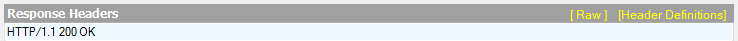
\includegraphics[width=\textwidth]{Pictures/test/AddAccountOK.png}
		\caption{OK}
		\label{fig:AddAccountOK}
	\end{subfigure}
	% 2
	\begin{subfigure}[b]{\textwidth}
		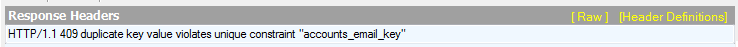
\includegraphics[width=\textwidth]{Pictures/test/AddAccountduplicate.png}
		\caption{Duplicate Key}
		\label{fig:AddAccountduplicate}
	\end{subfigure}
	% 3
	\begin{subfigure}[b]{\textwidth}
		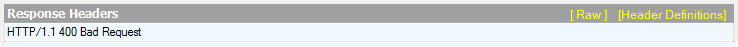
\includegraphics[width=\textwidth]{Pictures/test/AddAccountbadrequest.png}
		\caption{Bad Request}
		\label{fig:AddAccountbadrequest}
	\end{subfigure}
	% 4
	\begin{subfigure}[b]{\textwidth}
		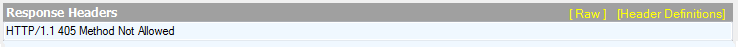
\includegraphics[width=\textwidth]{Pictures/test/AddAccountmethodnotallowed.png}
		\caption{Method Not Allowed}
		\label{fig:AddAccountmethodnotallowed}
	\end{subfigure}
	% 5
	\begin{subfigure}[b]{\textwidth}
		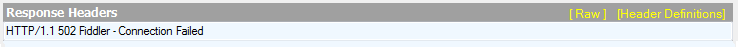
\includegraphics[width=\textwidth]{Pictures/test/AddAccountconnectionfailed.png}
		\caption{Connection Failed}
		\label{fig:AddAccountconnectionfailed}
	\end{subfigure}
	\caption{Results gathered from testing AddAccount}
	\label{fig:addaccountresults}
\end{figure}

\paragraph{OK}
In this case, the desired functionality is for the backend to insert a new row in the database-table called accounts, with the content specified in JSON-format listed in the composer figure \ref{fig:composeraddaccount}. 

For the given response message, see figure \ref{fig:AddAccountOK}, which is indeed the desired result and the test-case succeeded.
\paragraph{Duplicate Key}
In this case, the desired functionality is for the backend to detect that there already exists a row in the database with the same data as the one entered in the composer figure \ref{fig:composeraddaccount}. This will for an account only be possible for attributes marked with the UNIQUE identifier. In this case, it can only be the \texttt{email}, because the \texttt{accountid} is assigned by the database itself. This error was generated by executing the exact same HTTP request which has just returned an HTTP header with the OK result.

For the database violations, multiple types of database error-messages can occur, allowing for easy detection of the error made by the developer.

For the given response-message, see figure \ref{fig:AddAccountduplicate}, this is indeed the desired result and the test-case succeeded.
\paragraph{Bad Request}
In this case, the desired functionality is for the backend to tell the developer that they entered a bad request. This error can be generated in two ways. The first can be generated by corrupting the JSON formatting. This mean the standard for JSON-formatting was violated, which the backend should detect. The second error can be generated by changing the application/json in the composer figure \ref{fig:composeraddaccount} to application/xml. This means that the request body must be formatted as xml, which it obviously is not, hereby the error.

For the given response-message, see figure \ref{fig:AddAccountbadrequest}, this is indeed the desired result and the test-case succeeded.
\paragraph{Method Not Allowed}
The Web Service defined the type of \texttt{AddAccount} to be POST. Defining the HTTP requests to be any other type will result in the Method Not Allowed error. This error can be generated by changing the method-type to any other type than POST.

For the given response-message, see figure \ref{fig:AddAccountmethodnotallowed}, this is indeed the desired result and the test-case succeeded.
\paragraph{Connection Failed}
We turned the API off and executed an HTTP request trying to access the API. This should result in the connection failed error. 

For the given response-message, see figure \ref{fig:AddAccountconnectionfailed}, this is indeed the desired result and the test-case succeeded.

\subsection{GetRecipeById}
A few cases did not initially provide the expected results. The most interesting case of this happening was with the method called \texttt{GetRecipeById}.
This request returns a targeted recipe from the database, given that the provided ID exists in the database. During the early stages of the web service implementation, we had a strange error occur on the client side (running Java). The program kept throwing an exception: \texttt{java.net.SocketException: ECONNRESET (Connection reset by peer)}\cite{socketexception}. The exception basically says that the connection was terminated by the host, without returning an answer. This was strange because the web service was supposed to return a recipe if the ID existed or respond with HTTP status code 204 (No Content), if it did not exist. The error occurred because the web service did not properly get told by the \texttt{DBController} that it did not find a recipe with the provided ID, and when the web service stood without a recipe to return, as well as no confirmation that no such recipe existed, it just terminated the connection to the client. We fixed the error by altering the way the \texttt{DBController} handles empty queries, and as a result, it will now properly inform the client with 204 No Content.




%conclusion chapter%
\chapter{Conclusion}
\label{chap:conc}

The final product has turned out somewhat functional. It is able to provide suggestions based on user preferences and allows for easily obtained information about nearby stores and retailers. The problem statement described in \ref{sec:probstate} has in the clearest meaning been solved as the application is able to provide suggestions based on the preferences set by the specific user. It is however not ideal that the only preference to set at this given moment is monetary. The application could be greatly improved by having support for more preferences with more diversity so the target group could be broadened. We have, as mentioned, made it possible for each user to determine what the ideal radius for shopping is for them - this is perfect for fitting all target groups when it comes to means of transportation, whether by car, walking or other.

It should be noted that while serving recommendations are completely possible, the final product suffers greatly from a lack of data. At this point there are no available recipes unless entered manually, ingredients only from offers and statistics, and this makes it hard to actually make good recommendations.
Furthermore, we wanted to tag recipes to provide a form of meta-data that would improve the recommendation system, but again, this kind of information proved difficult to obtain without entering it manually.

The backend have been developed with performance in mind. We have intentionally created some suboptimal spacial entities with the purpose of making certain queries faster. These queries are generally the ones used by the application, meaning that these queries are likely to be run often. The backend does however spend some time making the calculations depending on how many recipes are in the database. The database was made accessible through a RESTful webs service API, which was found to work very well. It was easy to access from the application, and also great at abstracting the database away. From the backend side, extensive error handling is provided, meaning that if something should go wrong, the backend can recover, and will provide proper error messages for the application to deal with. The application is however responsible for handling cases where something goes wrong, but was not implemented in time. This makes the clients communication naive and have close to no error handling, this means the application is likely to crash because of not receiving the data it anticipated.

The application is unfinished although runnable. It could most definitely use some polishing and new graphics, as the graphics currently used are purely android studio sprites. There are both unfinished components, visuals and elements that needs refinement. It is however able to provide an intuitive way of getting recommendations through ones own preferences, along with browsing the contents of a recipe. The goal of making it user-friendly, feature rich and stable was mostly met. Features are limited given the limited project period, but extensive enough to provide a somewhat useful application. A lot of thought has gone into the usability of the application, and as result it feels easy to use.

\section{Evaluation}
\label{sec:eval}

The following paragraph will evaluate on the before mentioned conclusion. It gives more in depth evaluation than the conclusion, and digs deeper into the problematics several aspects of the program entails.

\paragraph{Recommender System}
\label{para:recommend}

The recommendation system, based on preferences is described in section \ref{sec:searchbypref}. The system has some obvious flaws that can be worked around, however designing a system like this is all about trade-offs. Our system could however be improved without introducing new trade-offs, as per right now the system gives a flat value based on its position in a sorted list (by the specific value). This creates scenarios where the actual value does not matter as much, imagine a recipe for which a retailer has an absurdly cheap offer compared to all the others. This recipe will be given a value of 100, while the next recipe which might be substantially more expensive, will be given a value of 99 or even 100 as well. While the system we have created does give a larger rating to the a cheaper offer, it does not give a proper representation of the relationship between values.

A way to solve this could be by implementing a standard deviation solution. It would be possible to give points based on how much a retailers offer differs from the actual average of the entire bunch of offers. This would make a lot more sense as the points given really reflect the value rather than the position of the value in a sorted list.

\subsection{Backend}
\label{subsec:evalbackend}
\paragraph{RESTful Web Service}
The web service performs very well and fulfills the purpose it was designed for. It offers a total of 46 HTTP requests to the client and completely hides away complex database functionality, as well as return useful computational results for the client like the results from the recommendation system. 

The web service is well structured and has been split into self-documenting interfaces responsible for very separated parts of the backend. Following this strict name-convention, it should be clear for the developer using the web service what a specific request should return. If something goes wrong, they are provided with a informative error-message, as can be seen in section \ref{chap:test} regarding test. 

In this project the web service does not fully receive the recognition it deserves. This is due to the uniform interface is provides, which is completely platform independent, meaning that this backend could serve iOS, windows phone or in this case android applications without alterations. This goal was part of the initial design decisions for the RESTful web service, because we wanted to develop a long-term realistic solution instead of hard-coding Android-specific responses based on an ad-hoc developed interface. This was not attractive for this project and complements the creation of the web service.

One of the only downsides to the RESTful web service is the lack of performance testing. We designed the backend with a purpose for fast query-handling and wanted to decrease the time a user spends waiting for results in the application. We never reached a goal with the data management that allowed us to proceed into this type of testing. The amount of data stored would simply not reflect the correct query time and the response-time through the web service would not be realistically used to say anything about the performance measures.

\paragraph{Data Management}
This project is highly dependent on the use of good and valid data. The data management has been prioritized very important which is why so many resources has been spent making the right decisions with the database. We wanted to avoid having to redesign the database because so much other functionality relies on it and is built on top of it. The RESTful web service HTTP requests are functioning purely as gateway to the database, and database changes cascades through the entire backend and requires extensive alterations, also to the web service. 

We coded an approximately 700 line long \texttt{DBController}, which handles all the desired database queries in this project. Had this project continued, we would spend time looking upon these queries and performance-optimizing them to deliver the fastest results possible to the user. Due to the limited resources in this project, we decided to lay aside the optimization until we had realistic data and application usage to work with. 

We only had to make two minor adjustments to the initial database design in this project. Because we spent so many resources designing it, we were able to keep the number of adjustments this low. The first adjustment we had to make was removing tags from recipes and ingredients themselves and making this as a weak-entity type, allowing easier and faster querying using tags. The second adjustment was an update to the attributes on ingredients. We added three additional attributes called organic, fat, and fresh. Since we started working with the offers from eTilbudsavis\cite{etilbudsavis}, we found that adding these attributes would make querying for healthy or fresh food much easier. Therefore we implemented this update.

\paragraph{Completeness}
The backend as a data provider is fully functional, and it is easily possible to access the data through the web service. The problem with the backend is  getting the valuable data from the external sources, parsing the data correctly and storing in the database for the user to look at and use. This is the biggest downside to the backend in its current state.
\chapter{Frontend}
\label{chap:frontend}

Intro!



\section{Future Work}
\label{sec:future}

\subsection{Backend}

\paragraph{Improved recipe data}
Så man kan judge øko, sundt, hurtigt at lave osv.

\paragraph{Better ingredient matching}
Så man bedre kan matche tilbud til ingredienser

\paragraph{Improved recommendation system}
Så det tager højde for flere ting

\paragraph{Recommendation categories}
Support for andet end aftensmad - kager, desserter, forretter osv.

\paragraph{Indexing of database}
Efter bogstaver m.m.

\paragraph{Automation of system}
Auto-opdateringer af alting

\paragraph{Support for pictures}
Opskrifer og profilbillede.

\subsection{Frontend}

\paragraph{Inputting new recipes in GUI}

\paragraph{Retouching the visual styles}
Appen er tør og kedelig

\paragraph{Updating the Discover fragment}
Der skal noget søgefunktion og noget til.

\subsection{Other}

\paragraph{Researching price data}
Find flere kilder, eller lav crowdsourcing på brugere.




%INSERT REPORT HERE%
%INSERT REPORT HERE%



% % % % % % % % % % % % % % % %

\bibliographystyle{chicago}
\bibliography{Litterature/litteratur}

% Appendix
\appendix
\chapter{SQL Query To Create Database}
\label{appendix:createdatabase}
The SQL query is displayed on the following page.
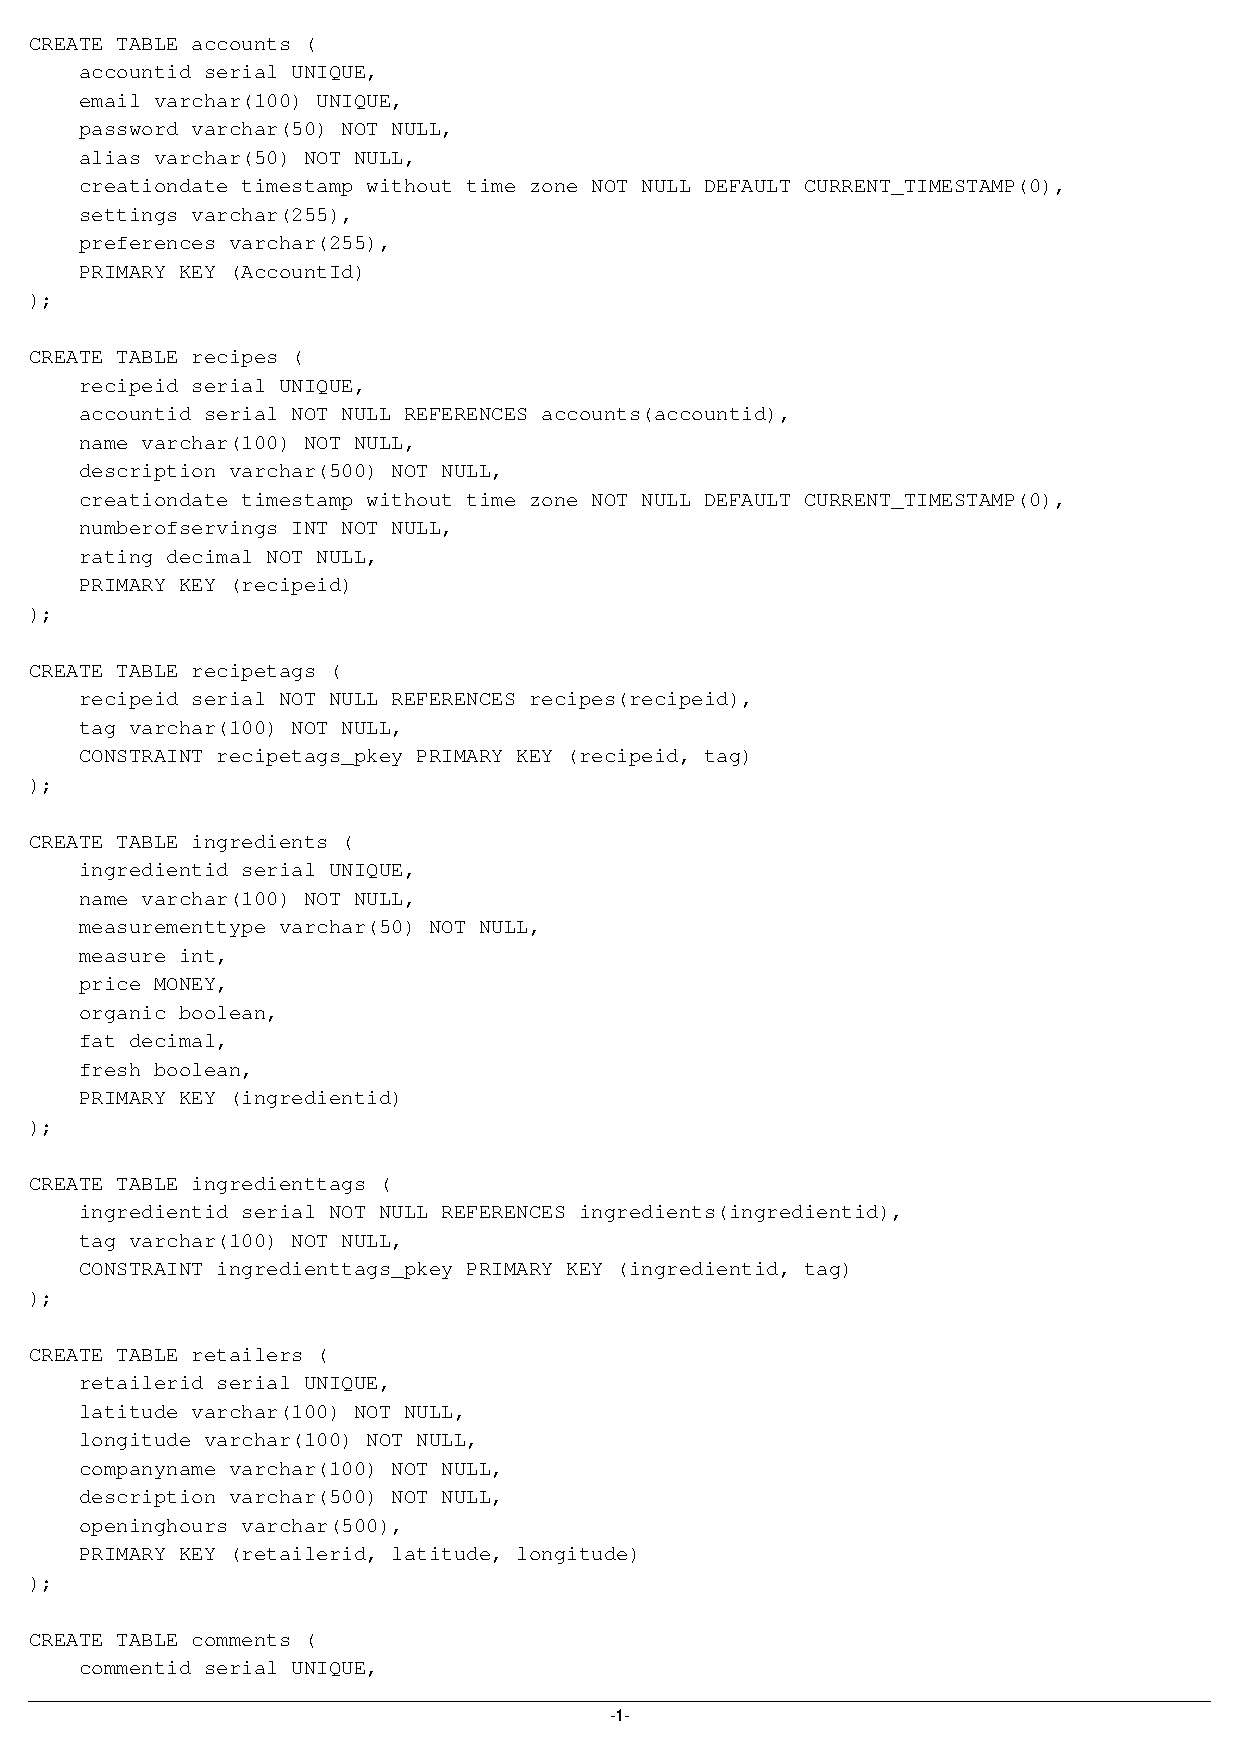
\includepdf[pages={1-2}]{appendix/dbcreation.pdf}



\label{LastPage}
\end{document}